\documentclass[output=paper]{LSP/langsci}
\author{Steven Doms}
\title{Non-human agents in subject position: {T}ranslation from {English into Dutch}: A corpus-based translation study of “give” and “show”}
\abstract{In English, sentences with action verbs like \textit{give} or \textit{show} can have non-human subjects that play the agent role. Non-human instances of agents are, however, less frequently attested in Dutch \citep[see e.g.][]{Delsoir2011, Vandepitte2011}. Dutch seems to impose restrictions on non-human instances, which do not contain all five proto-agent properties proposed by \citet{Dowty1991}. Hence, I expect that translators will not (always) translate English non-human agents as subjects of \textit{give} and \textit{show} with Dutch non-human agents as subjects of the Dutch cognates of \textit{give} and \textit{show}, \textit{geven} and \textit{tonen}, respectively. The choices translators make are described both on a syntactic and semantic level. The translation data of source-text sentences with \textit{give} and source-text sentences with \textit{show} are compared as to verify whether these source-text verbs give rise to different solutions proposed by translators.}
\maketitle
\rohead{\thechapter\hspace{0.5em}Non-human agents in subject position} % Display short title

\begin{document}

\section{Introduction}
English sentences such as (\ref{ex:5:1}a) and (\ref{ex:5:2}a) contain multiple participants, of which only one participant, to wit the agent, fulfills the grammatical function of subject and performs the action denoted by the verb \textit{give} and \textit{show}, respectively. In (\ref{ex:5:1}a), two other participants can be discerned apart from the non-human agent (\textit{an agreement which}): a recipient who receives something from the agent (\textit{Interbrew}) and a theme which is given to the recipient by the agent (\textit{a 24\% stake in China’s fifth largest and most profitable brewer}). In total, this example counts three participants, making it a trivalent sentence. Example (\ref{ex:5:2}a), on the other hand, exemplifies a divalent sentence with a non-human agent (\textit{Studies in animals}) and a theme (\textit{reproductive toxicity}). All examples given in this paper are taken from the Dutch Parallel Corpus (\textsc{dpc}) \citep[see][]{Rura2008}, except indicated otherwise. Subjects are marked in bold and verbs are underlined.

\exewidth{11}

\ea \label{ex:5:1}
  \ea 
  (\dots) an \src{agreement}{\textbf{agreement}}  which \ul{gives} \src{Interbrew}{Interbrew} a 24\% stake in \src{China}{China}'s fifth largest and most profitable brewer. 
  \ex Met de \target{agreement}{ondertekening} van deze overeenkomst\,{\dots}\,\ul{verwerft}\,{\target{Interbrew}{\textbf{Interbrew}}}\hspace*{-12mm}\,\\ 	een particpatie van 24\% in \target{China}{China}'s vijfde grootste brouwer \\
with the signature of this agreement (\dots) Interbrew acquires a particpation of 24\% in China's fifth largest brewer
  \z 
\z 
\connect{agreement} 
\connect{Interbrew}
\connect{China}

\exewidth{(23)}

\ea \label{ex:5:2}
 \ea \src{animal}{\textbf{Studies in animals}} \ul{have shown} \src{toxic}{reproductive toxicity} 
\\[1em]
\ex Uit \target{animal}{experimenteel onderzoek bij dieren} is   \target{toxic}{\textbf{reproductietoxiciteit}}  \ul{gebleken}\\
from experimental research on animals \textbf{reproductive toxicity} \ul{has become apparent}
  \z
\z

\connect{animal}
\connect{toxic}
%\begin{figure}
%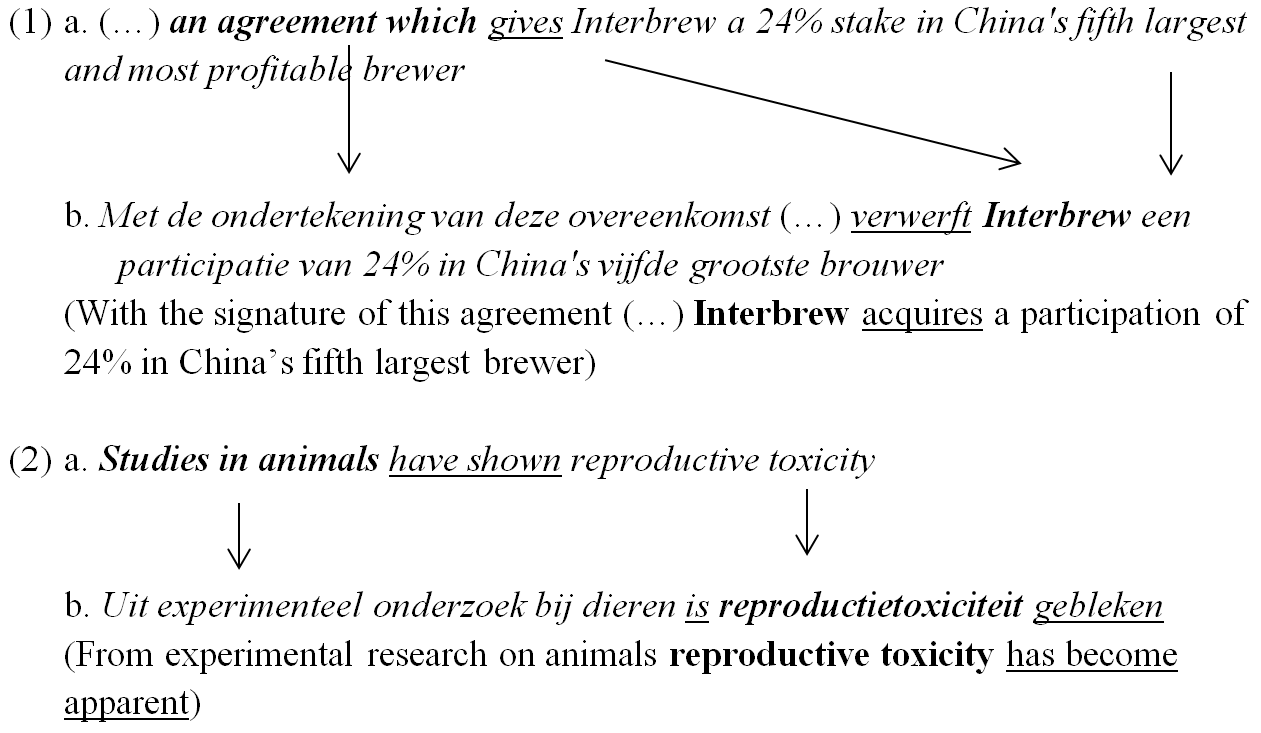
\includegraphics[width=1\textwidth]{./figures/S-1.png}
%\end{figure}

The English sentences display a non-human agent in subject position. Their Dutch translations in (\ref{ex:5:1}b) and (\ref{ex:5:2}b), however, do not. In (\ref{ex:5:1}b), the subject (\textit{Interbrew}) plays the role of recipient and refers to the source-text recipient. Further, the source-text non-human agent becomes an instrument (\textit{met de ondertekening van deze overeenkomst}), while the source-text theme remains a theme in the Dutch translation. This perspective-change in (\ref{ex:5:1}b) is achieved by the introduction of the reception verb \textit{verwerven} (\textit{acquire}) in Dutch. A different perspective-change is attested in (\ref{ex:5:2}b), in which the source-text non-human agent (\textit{studies in animals}) is represented as the prepositional object \textit{uit experimenteel onderzoek bij dieren} (\textit{from experimental research on animals}), indicating the origin of a state-of-affairs denoted in this target-text sentence. The source-text theme (\textit{reproductive toxicity}) becomes the target-text subject (\textit{reproductietoxiciteit}), which fulfills the theme role, typical of subjects of state verbs like \textit{blijken uit} (\textit{become apparent from}).

In this paper, I will investigate how 388 English sentences with non-human agents as subjects of \textit{give} or \textit{show} are translated into Dutch. From a linguistic point of view, I will enquire which solutions are chosen by translators to avoid Dutch non-human agents. From a translation perspective, Dutch translations of source-text sentences with \textit{give} and source-text sentences with \textit{show} are analyzed separately to verify whether the source-text verb impacts the translation choices opted for by translators. First, however, the concept of non-human agent is described and enclosed in the agent prototype in Section 2. 

\section{Agents} \label{sec:5:2}

Agents are participants which perform the action described by particular verbs. In the literature, agents have often been characterized in terms of so-called agentive features which according to \citet[49]{Hundt2004} “entail animacy (or even humanness)”, an example of which can be found in \citeauthor{Dowty1991}'s \citeyear{Dowty1991} theory of prototypical agents (see \sectref{sec:5:2:1}). Non-human instances of the agent role, however, do usually not represent these agentive features, which marks them as less prototypical agents. In \sectref{sec:5:2:2}, I will zoom in on these non-human agents and their properties. 

\subsection{Prototypical Agents} \label{sec:5:2:1}
In his \textit{Thematic Proto-Roles and Argument Selection}, \citet[572]{Dowty1991} proposes five features for prototypical agents:

\begin{itemize}
\item “volitional involvement in the event or state”
\item “sentience (and/or perception)”
\item “causing an event or change of state in another participant”
\item “movement (relative to the position of another participant)”
\item “exist independently of the event named by the verb”
\end{itemize}

These features can be summarized as volition, sentience, causation, movement and independent existence. Agents which have all five proto-agent properties listed by \citet{Dowty1991} are considered prototypical agents like \textit{John} in (\ref{ex:5:3}a), in which I assume that \textit{John} acts volitionally and sentiently. This trivalent sentence also includes a recipient (\textit{her}) and a theme (\textit{the book}), so that causation and movement are attested, both of which are related to participants other than the agent. Finally, the agent exists independently of the event in (\ref{ex:5:3}a), making it fulfill all five proto-agent properties.

In (\ref{ex:5:3}b), however, \textit{Kim} is not an instantiation of a prototypical agent. Although the properties volition, sentience and independent existence are found, causation and movement are not, because the divalent example in (\ref{ex:5:3}b) does not contain a recipient. The non-human agent (\textit{the book}) which is the subject of (\ref{ex:5:3}c) implies only the proto-agent feature independent existence. Causation and movement fail, because no recipient is attested, while volition and sentience, indeed, seem to be linked to human instances of the agent role.\newline 

\ea \label{ex:5:3}
\ea \textbf{John} \textit{gave} her the book yesterday.
\ex \textbf{Kim} \textit{gave} blood for the first time yesterday.
\ex \textbf{The book} \textit{gave} an overview of historic events in the 21st century.
\z
\z

%\noindent(3)
%\begin{enumerate}[a)]
%\item \textbf{John} \textit{gave} her the book yesterday. 
%\item \textbf{Kim} \textit{gave} blood for the first time yesterday. 
%\item \textbf{The book} \textit{gave} an overview of historic events in the 21st century.
%\end{enumerate}

The examples in \REF{ex:5:3} illustrate that both human and non-human agents can be instances of less prototypical agents. Non-human agents, however, are per definition less prototypical, because they do not display agentive features such as volition and sentience, which are typical of (some) human agents. In the next section, central attention is given to non-human instances of the agent role.

\subsection{Non-Human Agents} \label{sec:5:2:2}

In the literature, non-human subjects of action verbs have not always been treated as agents. Several authors \citep[see e.g.][]{Fillmore1968,Quirk1972,Levin1993} consider some of these subjects as instances of the instrument role. \textit{The door} in (\ref{ex:5:4}a-b) exemplifies such an instrument that can become subject in sentence (\ref{ex:5:4}b), in which there is no agent.

\ea \label{ex:5:4}
\ea \textbf{Dennis} \textit{opened} the door with the key.
\ex \textbf{The key} \textit{opened} the door. 
\z
\z

Other linguists \citep[see e.g.][]{Biber1999,Talmy2000} discern what they call causers, i.e. abstract entities and (natural) forces such as a \textit{biting wind gusting to 30 knots} in \citeauthor{Biber1999}’s (\citeyear{Biber1999}) example in \REF{ex:5:5}.

\ea \label{ex:5:5}
\ea \textbf{A biting wind gusting to 30 knots} \textit{threatened to blow} the fragile, 15-ft fiberglass hydroplane off course.
\z
\z

In this paper, non-human subjects of action verbs are seen as agents. The agent role is defined as the participant which is the subject of an action verb and which – following \citet{Dowty1991} – exists independently of the event named by that action verb. This definition of agent allows for a concept of agents/agency which does not a priori presuppose animacy or humanness of the agent role. Hence, the agent role can be further subdivided into human and non-human instances. The source-text non-human agents which are under investigation are subjects of the English action verbs \textit{give} and \textit{show}. How these source-text non-human agents are translated in Dutch is shown in \sectref{sec:5:6}. First, however, an account is made of restrictions on non-human agents which seem to exist in Dutch according to earlier research.

\section{Constraints on Dutch non-human agents} \label{sec:5:3}
In some languages, restrictions have been shown to exist on non-human agents as subjects of typical action verbs. This has, for instance, been demonstrated for German \citep[see e.g.][]{Bahns1993}, Spanish \citep[see e.g.][]{Slabakova2002} and some Asian languages \citep[see e.g.][]{Master1991}. Recently, studies have been conducted to determine whether such constraints also exist in Dutch. In this section, the focus lies on four recent studies in which Dutch translations of English non-human agents have been investigated.

The first study to be discussed here originates from  \citet{Vandepitte2007}, who focuses on the translation techniques one particular translator used in translating 300 English sentences containing a non-human agent into Dutch. These source-text and target-text sentences were part of an approximately 70,000 word parallel corpus which was compiled from Hertz’s \textsc{essay} \textit{The Silent Takeover} and its Dutch translation \textit{De Stille Overname}. Vandepitte distinguishes between four translation techniques: \textit{no semantic or pragmatic differences between source and target text, implicitation} (i.e. those cases in which the target-text sentence is more implicit than the source-text sentence), \textit{explicitation} (i.e. those cases in which the target-text sentence is more explicit than the source-text sentence) \textit{and other semantic or pragmatic changes}, which is in most instances a combination of both implicitation and explicitation.

Vandepitte reports that in about one third of the Dutch translations, no semantic or pragmatic differences are attested between source-text and target-text sentences. Two thirds of the translations, on the other hand, display shifts. Explicitation occurs in less than one out of ten target-text sentences, whereas one out of four target-text sentences can be seen as an instance of implicitation. About one third of the 300 instances examined by \citet{Vandepitte2007} show other semantic or pragmatic changes. These results reveal that translation of non-human agents into Dutch leads to (especially) semantic and (sometimes) pragmatic changes. This study, however, does not zoom in on the semantics of the non-human agents themselves, as opposed to \citeauthor{Dhaeyere2010}'s (\citeyear{Dhaeyere2010}) inquiry. 
	

D’haeyere identifies “non-prototypical agents with prototypical agent requiring predicates”, which are abbreviated as \textsc{npaparp}s, a term coined by \citet{Vandepitte2010}. These abstract and non-human agents as subjects of verbs that typically take a human agent are searched in a set of 200 English sentences. The way in which these English source-text sentences are translated in Dutch is investigated in order to establish whether Dutch non-human agents are avoided. \citet{Dhaeyere2010} discerns three possible ways in which translators can deal with \textsc{npaparp}s: similar translation of the \textsc{npaparp}, different translation of the \textsc{npaparp} or no \textsc{npaparp} in Dutch.  

Her findings suggest that in little more than half of all translations, translators opted to maintain the \textsc{npaparp}s in Dutch, in which cases the \textsc{npaparp}s were most often translated similarly and only sometimes different vis-à-vis the source text. In the other half of the instances, however, the Dutch translations no longer contained \textsc{npaparp}s. D’haeyere describes shifts which were used to avoid \textsc{npaparp}s in Dutch. In almost half of these instances, \textsc{npaparp}s are transformed into Dutch prepositional phrases, i.e. into translations which do no longer contain a verb, but a preposition which links the other lexical elements. Further, in about one out of ten Dutch translations \textsc{npaparp}s have disappeared, because copular verbs are used. Two other frequent shifts are the introduction of human agents and agent ellipsis. Finally, in some instances, the use of a state or content verb or a conditional clause are attested. 

D’haeyere’s results indicate that it is the verb that is adapted most often to avoid Dutch non-human agents. In those cases in which Dutch translations contain a non-human agent, mainly causative verbs like \textit{zorgen voor} (\textit{cause}) are found. Furthermore, D’haeyere’s data show that Dutch non-human agents more often refer to concrete objects, whereas more abstract entities are found in the source-text sentences.       

As opposed to \citet{Vandepitte2007} and \citet{Dhaeyere2010}, \citet{Vandepitte2011} do not focus on the product of translation, but on the translation process. In an experimental study, they inquire into the extent to which \textsc{npaparp}s result in higher translation processing costs than prototypical (human) agents. To verify this, a test is built which consists of seventy-six English sentences -- thirty-eight with a prototypical agent and thirty-eight with a non-prototypical agent -- which have to be translated in Dutch by trained (master students) and untrained (first-year bachelor students) translators. In total, twenty-four translators -- fourteen trained and ten untrained -- provide comparable results. The experiment shows that untrained translators translate English non-human agents with Dutch non-human agents in approximately 83\% of the instances, while trained translators maintain non-prototypical agents in about 73\% of the Dutch translations. 

Besides this “very strong tendency to translate constructions with a non-prototypical agent with a construction that similarly has a non-prototypical agent”, \citet[11]{Vandepitte2011} also find that English sentences with non-prototypical agents are translated slower by both trained and untrained translators, which makes them conclude that \textsc{npaparp}s constitute a translation process problem. 

Finally, \citet{Delsoir2011} used \citeauthor{Vandepitte2011}'s \citeyear{Vandepitte2011} data to investigate which \textsc{npaparp}s are accepted in Dutch and which are not. Delsoir has 226 respondents rate twenty-eight Dutch translations of English \textsc{npaparp}s in terms of acceptability. In total, nine translations are rated unacceptable, fourteen translations are found to be sufficiently acceptable and only five translations receive the label acceptable in Dutch. Delsoir argues that the Dutch verbs in the translations at least “partly have volition as a feature, and therefore should require a prototypical agent” \citet[34]{Vandepitte2011}, leading him to the conclusion that English has been leaking into Dutch on a grammatical level. 

The findings in these four studies are based on English source-text sentences and their Dutch translations which contain verbs belonging to different semantic verb types which typically call for very specific syntactic patterns. In the present study, however, the English source-text sentences only include two verbs: \textit{give} and \textit{show}, for each of which a detailed semantic and syntactic description is given in \sectref{sec:5:4}.  

\section{\textit{Give} and \textit{show}} \label{sec:5:4}

In this study, all source-text non-human agents are subjects of either \textit{give} or \textit{show}. \textit{Give} as well as \textit{show} typically calls for a human agent subject which conducts a (non-)material transfer of a theme to(wards) a recipient. These two trivalent verbs which are frequently attested in the Dutch Parallel Corpus (see also \sectref{sec:5:5}), however, also allow for non-human agents in subject position, as was illustrated by the examples in \REF{ex:5:1} and \REF{ex:5:2}, so that they are expected to yield sufficient English source-text sentences with non-human agents in subject position, of which the Dutch translations will be analyzed and compared. Both English verbs are treated in detail below.  
  
\subsection{\textit{Give}}

\textit{Give} is a trivalent verb which expresses an act in which an agent hands over a theme to a recipient. The agent initiates the action and typically becomes subject, while the theme has the grammatical function of direct object and the recipient is the indirect object, as was illustrated by example (\ref{ex:5:1}a) in the introduction. Although \textit{give} can call for three participants (agent, theme, recipient), it can also occur in sentences which portray only two participants (agent and theme, but no recipient), as in (\ref{ex:5:3}b-c). In \sectref{sec:5:2:1}, it has been demonstrated that the absence of the recipient has an impact on the prototypicality of the agent. Since in this paper I zoom in on one particular type of agent, i.e. the non-human agent, which can be considered an agent which includes only one of  the five proto-agent properties listed by \citet{Dowty1991}, I will not limit myself to instances with three participants. Both divalent and trivalent English source-text sentences with non-human agents as subjects of \textit{give} are taken into account.

\subsection{\textit{Show}}

The English verb \textit{show} resembles \textit{give} in that it allows for three participants: an agent, a theme and a recipient. In a trivalent sentence with \textit{show}, the agent shows the recipient a theme, as in the nominal relative clause in (\ref{ex:5:6}a), in which the non-human agent (\textit{one simple concept that}) fulfills the grammatical function of subject, the recipient (\textit{us}) is the indirect object and the theme (\textit{the way forward}) functions as grammatical direct object. The theme may occur as a noun phrase like in (\ref{ex:5:6}a), but can, for instance, also take the form of a \textit{that}-clause like in (\ref{ex:5:6}b). As it was the case for \textit{give}, \textit{show} can also be found in divalent sentences such as (\ref{ex:5:2}a), in which there is no recipient. Dutch translations of both divalent and trivalent sentences with \textit{show} are investigated.

\ea \label{ex:5:6}
\ea There is \textbf{one simple concept that} \ul{shows} us the way forward
\ex \textbf{The salon} \ul{showed} people that we did wash our hair
\z
\z

Before analyzing the Dutch translations of English source-text sentences containing \textit{give} and \textit{show}, the method of selecting the data underlying this study is presented in \sectref{sec:5:5}.

\section{Corpus: data and methodology} \label{sec:5:5}

In order to procure English source-text sentences with non-human agents as subjects of \textit{give} and \textit{show}, the lemmas “give” and “show” were searched in the 10 million word sentence-aligned Dutch Parallel Corpus (\textsc{dpc}) of English, French and Dutch \citep[see e.g.][]{Rura2008},\footnote{A search interface for the \textsc{dpc} was created by I. Delaere and A. Malfait, to whom I am greatly indebted} which comprises five text types: literature, instructive, journalistic, administrative texts and external communication. This search yielded 1986 English sentences with \textit{give} (1208) and \textit{show} (778) lemmas. Further filtering of these sentences was required. First, all English source-text sentences which did not have a Dutch translation – for reasons unknown to me – were left out as well as source-text sentences which occurred more than once with identical translations, in which case only one English-Dutch translation pair was maintained. Furthermore, source-text sentences were attested in which \textit{give} and \textit{show} did not denote the verb meanings described in \sectref{sec:5:4}. Hence, instances containing phrasal verbs (e.g. \textit{give in}, \textit{show up}), expressions (e.g. \textit{give someone the eye}, \textit{show one’s hand}) and idioms (e.g. \textit{give birth to}, \textit{show face}) were also filtered out. These first two filterings eventually leave us with 1220 instances.

Not all of these 1220 instances, however, have an agent as their subject. Passive sentences and source-text sentences without subjects (e.g. past participial, prepositional, infinitival clauses as well as nominalizations and adjectives) received the label “no agent”, as shown in \tabref{tab:5.1}. The other instances have a subject which represents the agent role. A difference was then made between source-text sentences with a human and a non-human agent. \tabref{tab:5.1} shows how often source-text sentences with \textit{give} and \textit{show} contained no, a human or a non-human agent.     

\begin{table}
     \centering
     \begin{tabularx}{\textwidth}{XXXXXXX}
     \lsptoprule
                  &  \textit{Give}   & \textit{\%}  & \textit{Show}  & \textit{\%} & Total & \textit{\%} \\ \midrule
       \textbf{No Agent}    & 376    & 48.3          & 98	           & 22.2      & 474   & 38.9 \\
       \textbf{Human Agent} & 248    & 31.9          & 110             & 24.9      & 358   & 29.3  \\
       \textbf{Non-Human Agent} & 154 & 19.8         & 234             & 52.9      & 388   & 31.8 \\  \midrule
       \textbf{Total}       & 778     & 63.8        & 442              & 36.2      & 1220  & 100  \\ 
  \lspbottomrule     
     \end{tabularx}
 
     \caption{Instances with and without agents}
     \label{tab:5.1}
     % Verweis im Text mittels \REF{tbl:beispieltabelle}
 
   \end{table}

The results in \tabref{tab:5.1} reveal that about half of the source-text sentences with \textit{give} do not include agents, while this is true for only about a fifth of the source-text sentences with \textit{show}. If the attestations of \textit{give} and \textit{show} in agentless instances are left out of consideration, both verb queries in the \textsc{dpc} seem to yield a comparable number of source-text sentences which are headed by agent subjects. \textit{Give}, however, preferably takes human agents as its subjects, whereas \textit{show} is attested especially with non-human agent subjects. In total, 388 instances, i.e. approximately a third of all attested source-text sentences, contain a non-human agent as subject of \textit{give} or \textit{show}. In \sectref{sec:5:6}, a detailed analysis is made of the ways in which these source-text sentences have been translated into Dutch. 

\section{Data analysis} \label{sec:5:6}

In these sections, I will elaborate on the Dutch translations of 154 source-text sentences with non-human agents as subjects of \textit{give} and 234 source-text sentences with non-human agents as subjects of \textit{show}. In \sectref{sec:5:6:1}, the way in which the source-text non-human agents are translated in Dutch is investigated. The choices translators make to avoid Dutch non-human agents are described in \sectref{sec:5:6:2}.
  
\subsection{Dutch translations of non-human agents} \label{sec:5:6:1}

As reported in \sectref{sec:5:3}, Dutch has been shown to have restrictions on non-human agents in subject position. In this section, Dutch translations of English source-text non-human agents are examined to determine how often English non-human agents as subjects of \textit{give} and\textit{ show} are translated with Dutch non-human agents. \tabref{tab:5.2} shows what happens with the 388 source-text non-human agents in Dutch translations.

\begin{table}
     \centering
     \begin{tabularx}{\textwidth}{XXXXXXX}
     \lsptoprule
                  &  EN non-human\newline agent: \textit{give}   & \textit{\%}  & EN non-human\newline agent: \textit{show}  & \textit{\%} & Total & \textit{\%} \\ \midrule
       \textbf{NL non-human agent}    & 92    & 59.7         & 130	          & 55.5      & 222   & 57.2 \\
       \textbf{NL human agent}        & 10    & 6.5          & 17             & 7.3       & 27    & 7  \\
       \textbf{NL no agent}           & 52    & 33.8         & 87             & 37.2      & 139   & 35.8 \\  \midrule
       \textbf{Total}                 & 154   & 39.7         & 234            & 60.3      & 388   & 100  \\ 
   \lspbottomrule    
     \end{tabularx}
 
     \caption{Dutch translations of English non-human agents}
     \label{tab:5.2}
     % Verweis im Text mittels \REF{tbl:beispieltabelle}
 
   \end{table}

As \tabref{tab:5.2} demonstrates, in about 57\% of the Dutch translations, non-human agents are attested in subject position. This number of Dutch non-human agents corresponds more or less to \citet{Dhaeyere2010} findings, which showed non-human agents in slightly more than half of 200 Dutch translations. Almost 60\% of the source-text sentences with \textit{give} result in Dutch translations with non-human agents, while almost 55\% of the source-text sentences with \textit{show} give birth to Dutch translations with non-human agents.

In all these instances, the source-text non-human agents have been translated literally or similarly into Dutch and the source-text verbs \textit{give} and \textit{show} have been translated with their Dutch cognates \textit{geven} or \textit{tonen}, as in (\ref{ex:5:7}b) and (\ref{ex:5:8}b), or with other Dutch action verbs like \textit{bieden} (\textit{offer}) in (\ref{ex:5:9}b) or the Dutch verbal collocation \textit{in kaart brengen} (\textit{map out}) in (\ref{ex:5:10}b) which typically call for an agent as their subject.      

\ea \label{ex:5:7}
\ea
\textbf{The} \src{annualreport}{\textbf{annual report}} \ul{gives} a true and fair view of the \src{results}{results} of the company
\ex
\textbf{Het} \target{annualreport}{\textbf{jaarverslag}} \ul{geeft} een getrouw overzicht van de \target{results}{resultaten} van het bedrijf\\
\textbf{the annual report} \ul{gives} a true overview of the results of the company
\z
\z

\connect{annualreport}
\connect{results}


\ea \label{ex:5:8}
\ea
\textbf{An} \src{xray}{\textbf{x-ray}} \ul{showed} two \src{foreignbodies}{foreign bodies}\\[1em]
\ex \textbf{Een} \target{xray}{\textbf{röntgenfoto}} \ul{toonde} twee \target{foreignbodies}{vreemde objecten}\\
\textbf{an x-ray} \ul{showed} two foreign objects
\z
\z

\connect{xray}
\connect{foreignbodies}

\newpage
%\begin{figure}
%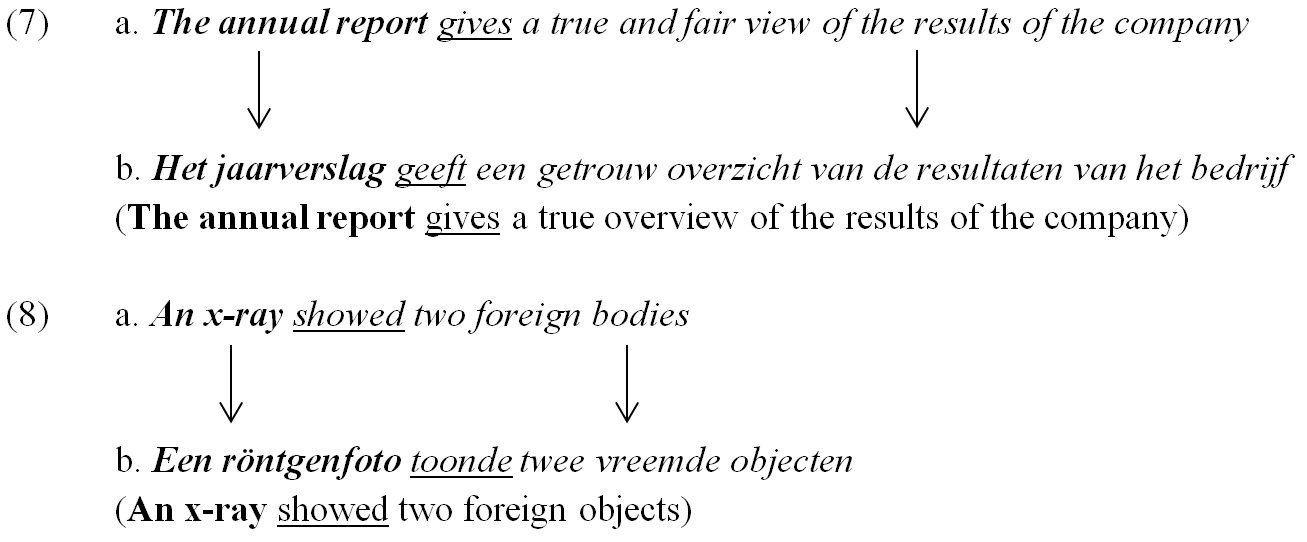
\includegraphics[width=1\textwidth]{./figures/S-2.png}
%\end{figure}


\ea \label{ex:5:9} 
\ea
\textbf{The} \src{expo}{\textbf{World Expo}} \ul{gives} \src{us}{us} the \src{chance}{chance} to meet customers\\[1em]
\ex
\textbf{De} \target{expo}{\textbf{Wereldexpo}} \ul{zal} \target{us}{ons} de \target{chance}{mogelijkheid} \ul{bieden} bestaande klanten te ontmoeten\\
\textbf{the World Expo} \ul{will offer} us the possibility to meet existing customers
\z
\z

\connect{expo}
\connect{us}
\connect{chance}

\ea \label{ex:5:10}
\ea
\textbf{Our} \src{study}{\textbf{study}} \ul{shows} for the first time the \src{process}{entire process}\\[1em]
\ex
\textbf{Onze} \target{study}{\textbf{studie}} \ul{brengt} voor de allereerste keer het \target{process}{hele proces} \ul{in kaart}\\
\textbf{our study} \ul{maps out} for the very first time the entire process
\z
\z

\connect{study}
\connect{process}

%\begin{figure}
%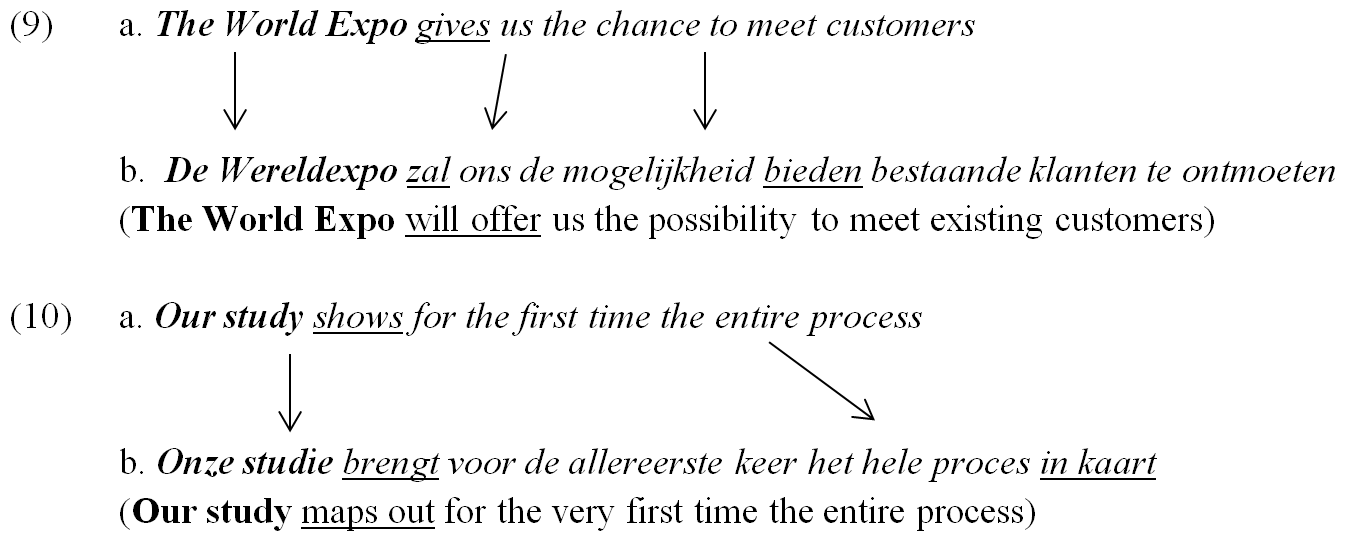
\includegraphics[width=1\textwidth]{./figures/S-3.png}
%\end{figure}

Although translators have opted for verbs which typically take agents as their subjects, only 7\% of the Dutch translations have a subject that plays the agent role and at the same time refers to a human referent. If translators did decide to avoid Dutch (non-human) agents, other solutions were chosen. These solutions which lead to Dutch translations without non-human agents are illustrated and given center stage in the next section.  

\subsection{Dutch translations without non-human agents} \label{sec:5:6:2}
More than forty percent of all Dutch translations include a subject that is not a non-human agent. Translators have produced very diverse translations which can be grouped here as three main solutions to avoid Dutch non-human agents: introduction of a human agent, use of a non-agentive subject or omission of the verb. \tabref{tab:5:3} shows how often translators used each of these solutions. 

\begin{table}
     \centering
     \begin{tabularx}{\textwidth}{XXXXXXX}
     \lsptoprule
                  &  EN non-human\newline agent: \textit{give}   & \textit{\%}  & EN non-human\newline agent: \textit{show}  & \textit{\%} & Total & \textit{\%} \\ \midrule
       \textbf{NL non-human agent subject}  & 10          & 16.1     & 17	          & 16.4      & 27   & 16.3 \\
       \textbf{NL non-agentive subject}     & 47          & 75.8     & 75             & 72.1       & 122   & 73.5  \\
       \textbf{NL no verb}           & 5    & 8.1         & 12       & 11.5       & 17   & 10.2 \\  \midrule
       \textbf{Total}                & 62   & 37.3        & 104      & 62.7       & 166   & 100  \\ 
       
     \lspbottomrule
     \end{tabularx}
 
     \caption{Solutions used to avoid NL non-human agents}
     \label{tab:5:3}
     % Verweis im Text mittels \REF{tbl:beispieltabelle}
 
   \end{table}

As \tabref{tab:5:3} indicates, translators’ choice to avoid Dutch non-human agents mainly results in target-text sentences with a non-agentive subject. Both the introduction of a Dutch human agent (in about 16\% of these translations) and omission of verb in Dutch (in about 10\% of these translations) explain what happens in the remaining quarter of the Dutch translations without non-human agents in subject position. All three solutions have different ways of realization which are dealt with in the following sections. In \sectref{sec:5:6:2:1}, instances with Dutch human agents are discussed in detail, while \sectref{sec:5:6:2:2} zooms in on instances with Dutch non-agentive subjects. In \sectref{sec:5:6:2:3}, Dutch translations without a verb are dealt with.  

\subsubsection{Introduction of a human agent} \label{sec:5:6:2:1}

A first solution adopted by translators in less than one in ten translations (see \tabref{tab:5.2} and \tabref{tab:5:3}, \sectref{sec:5:6:1} and \sectref{sec:5:6:2}) consists of introducing a Dutch human agent. This solution can be realized in two different ways. Either translators translate source-text sentences literally (or similarly), except for the source-text non-human agent which is replaced with a human(ized) agent in Dutch, like \textit{institutional} “\textit{power-grabbing}” in (\ref{ex:5:11}a) which is translated with the collective noun \textit{instellingen} (\textit{institutions}) in (\ref{ex:5:11}b) or like the \textit{pictures} which become \textit{hij} (\textit{he}), thus unveiling the metonymic relation between a product in (\ref{ex:5:12}a) and its producer in (\ref{ex:5:12}b).  

\ea \label{ex:5:11}
\ea \textbf{Institutional} \src{grabbing}{\textbf{``power-grabbing''}} \ul{will give} the \src{convention}{Convention}\\ a \src{badname}{bad name}\\[1em]
\ex \textbf{Instellingen die} \target{grabbing}{``\textbf{machtsbelust}''} \textbf{optreden} \ul{geven} de \target{convention}{Conventie} een \target{badname}{slechte naam}\\
\textbf{institutions that act power-hungry} \ul{give} the Convention a bad name
\z
\z

\connect{grabbing}
\connect{convention}
\connect{badname}

\ea \label{ex:5:12}
\ea
\src{pictures}{\textbf{The pictures}} \ul{show} the \src{aftermath}{aftermath of the battle}\\[1em]
\ex \target{pictures}{\textbf{Hij}} \ul{toont} het \target{aftermath}{naspel van de veldslag}\\
\textbf{he} \ul{shows} the aftermath of the battle
\z
\z
\connect{pictures}
\connect{aftermath}

%\begin{figure}
%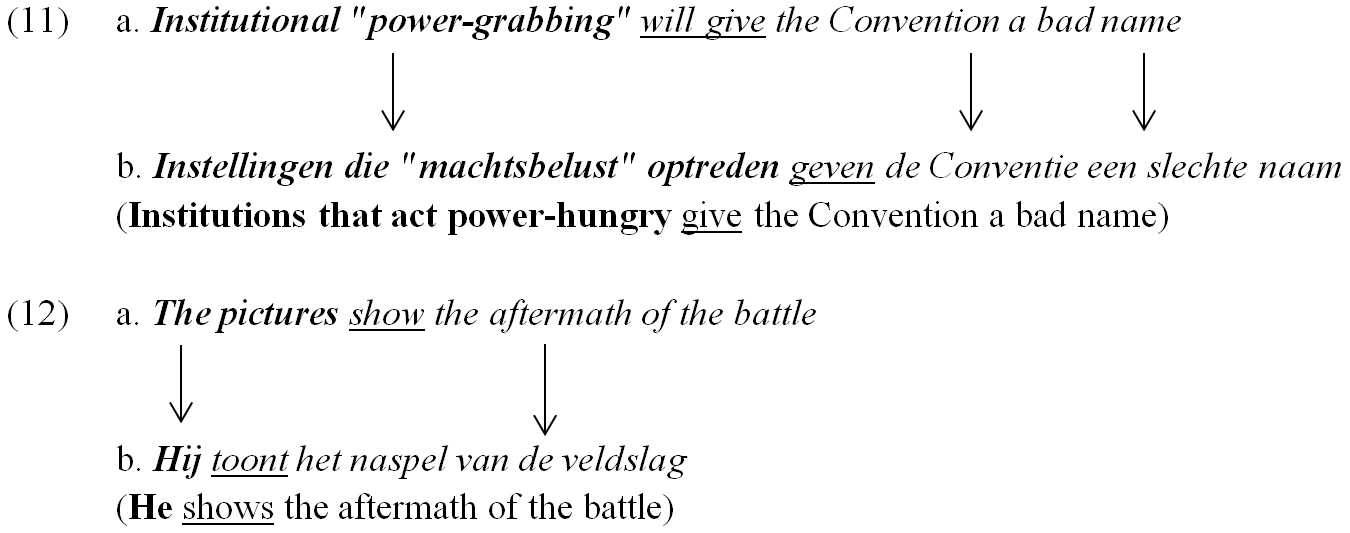
\includegraphics[width=.9\textwidth]{./figures/S-4.png}
%\end{figure}

In other instances, however, translators have not only introduced a human agent in the Dutch translations, but also replaced the source-text verb \textit{give} or \textit{show} with another action verb. In \REF{ex:5:13}, the source-text non-human agent \textit{this agreement} is translated as a prepositional object in Dutch, while the source-text recipient \textit{us} becomes the subject in the target text. This human subject plays the agent role of the Dutch verb \textit{verkopen} (\textit{sell}), which is preceded by the modal verb \textit{kunnen} (\textit{can}). In this instance, the source-text sentence is trivalent, whereas the target-text sentence only counts two participants. 

In \REF{ex:5:14}, the target-text sentence also reveals a human agent: \textit{een presentatrice met een grote hoofddoek} (\textit{a female presenter with a big headscarf}). The source-text subject, however, referred to the non-human agent \textit{the television} which occurs as an adverbial in the Dutch translation. The source-text verb \textit{show} has been replaced with Dutch \textit{lezen} (\textit{read}) which calls for a theme as its direct object, in this case \textit{het nieuws} (\textit{the news}) which was part of the source-text direct object, but solely becomes the target-text direct object. In this example, both source-text and target-text sentence exhibit a divalent structure. Although the divalent structure in both sentences is very different, all source-text elements are represented in the Dutch translation. This tendency can also be distilled from the two other solutions translators have opted for to avoid Dutch non-human agents in subject position.             

%\begin{figure}
%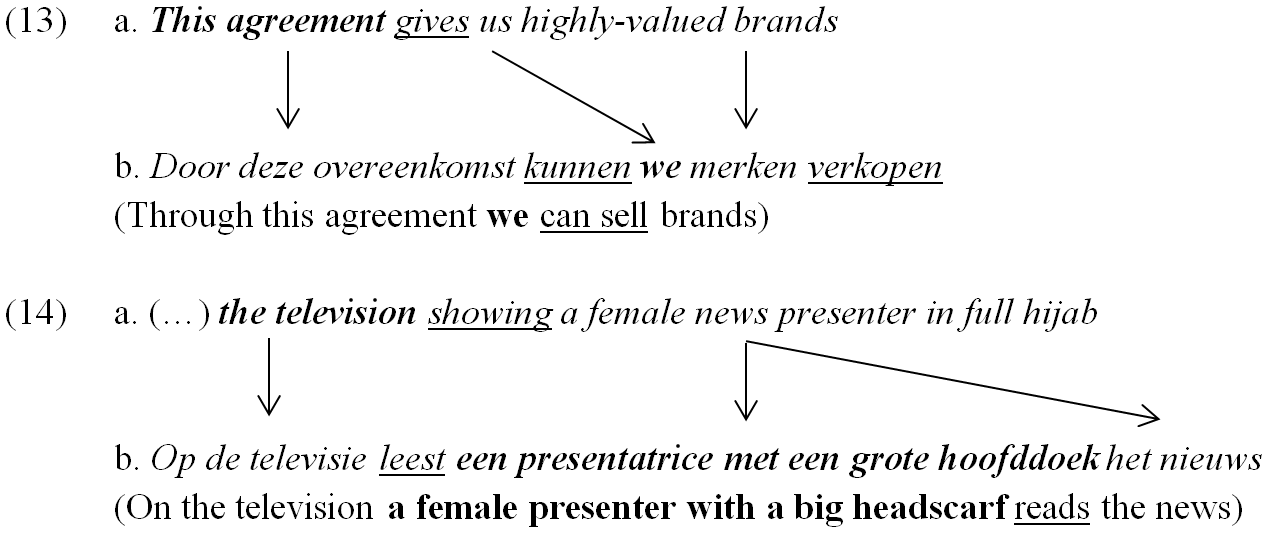
\includegraphics[width=1\textwidth]{./figures/S-5.png}
%\end{figure}

\ea \label{ex:5:13}
\ea
\textbf{This} \src{agr2}{\textbf{agreement}} \ul{gives} \src{us2}{us} highly-valued \src{brands}{brands}\\[1em]
\ex Door deze \target{agr2}{overeenkomst} \ul{kunnen} \target{us2}{\textbf{we}} \target{brands}{merken} \ul{verkopen}\\
through this agreement \textbf{we} \ul{can sell} brands
\z
\z

\connect{agr2}
\connect{us2}
\connect{brands}

\ea \label{ex:5:14}
\ea
(\dots) \textbf{the} \src{tv}{\textbf{television}} \ul{showing} a \src{fnp}{female \src{news}{news} presenter} in full hijab
\ex
Op de \target{tv}{televisie} \ul{leest} \textbf{een} \target{fnp}{\textbf{presentratrice}} \textbf{met een grote hoofddoek} het \target{news}{nieuws}\\[1em]
on the television \textbf{a female presenter with a big headscarf} \ul{reads} the news
\z
\z

\connect{tv}
\connect{fnp}
\connect{news}

\subsubsection{Use of a non-agentive subject} \label{sec:5:6:2:2}

In more than a third of all Dutch translations (see \tabref{tab:5.2}), translators choose a Dutch subject which does not play the agent role. Instead, these Dutch subjects denote the semantic role of another participant such as theme, possessor or recipient. \tabref{tab:5.4} shows how often each of these non-agentive roles occurred as subjects of Dutch translations.

\begin{table}
     \centering
     \begin{tabularx}{\textwidth}{XXXXXXX}
     \lsptoprule
     &  Source-text sentences\newline with \textit{give}   & \textit{\%}  & Source-text sentences\newline with \textit{show } & \textit{\%} & Total & \textit{\%} \\ \midrule
       \textbf{NL theme subject}  & 25    & 53.2      & 70	          & 93.3      & 95   & 77.9 \\
       \textbf{NL possessor subject}     & 7     & 14.9        & 5      & 6.7       & 12   & 9.8  \\
       \textbf{NL recipient subject}     & 15    & 31.9        & 0      & 0        & 15   & 12.3 \\  \midrule
       \textbf{Total}                    & 47    & 38.5        & 75     & 61.5       & 122   & 100  \\ 
\lspbottomrule
\end{tabularx}

     \caption{Dutch translations with non-agentive subjects}
     \label{tab:5.4}
     % Verweis im Text mittels \REF{tbl:beispieltabelle}
\end{table}
  

 
The non-agentive role that occurs most often as subject in these Dutch translations is theme. Especially in translations of source-text sentences with \textit{show}, theme subjects are very frequently attested. The introduction of Dutch theme subjects is achieved through two ways: either by using a Dutch state verb like \textit{zijn} (\textit{be}), as in (\ref{ex:5:15}b), or by using the passive voice, as in (\ref{ex:5:16}b), which gives rise to theme subjects as well.

\newpage

\ea \label{ex:5:15} 
\ea
\textbf{The} \src{doctrine}{\textbf{doctrine}} \ul{gave} a \src{yg}{younger generation} a\\\, \src{wot}{way of thinking}
\ex \target{doctrine}{\textbf{Rasta}} \ul{was} voor de \target{yg}{jongere generaties} een\\\, \target{wot}{nieuwe manier van denken}\\[1em]
\textbf{rasta} \ul{was} for the younger generation a new way of thinking
\z
\z

\connect{doctrine}
\connect{yg}
\connect{wot}

\ea \label{ex:5:16}
\ea \src{animalstudies}{\textbf{Animal studies}} \ul{have shown} that \src{exposure}{exposure} decreases\\[1em]
\ex
In \target{animalstudies}{dieronderzoeken} \ul{is anngetoond} \textbf{dat} \target{exposure}{\textbf{blootstelling}} \textbf{afneemt}\\
in animal studies \ul{it has been shown} \textbf{that exposure decreases}
\z
\z

\connect{animalstudies}
\connect{exposure}

%\begin{figure}
%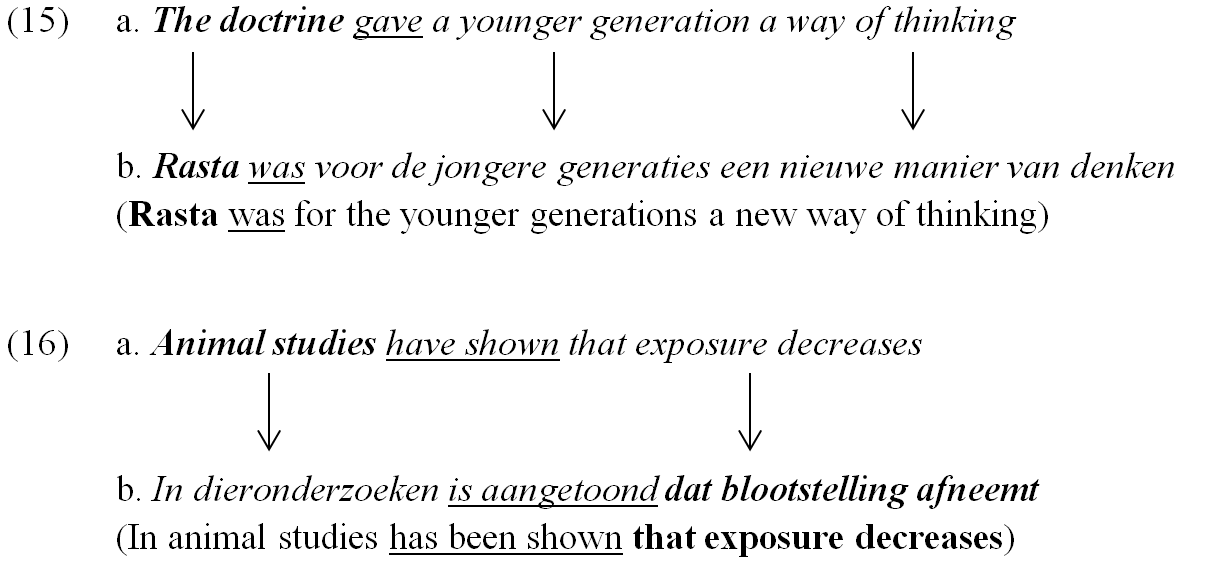
\includegraphics[width=1\textwidth]{./figures/S-6.png}
%\end{figure}

The target-text subject \textit{rasta} in (\ref{ex:5:15}b) refers to the source-text subject \textit{the doctrine}, but translator’s choice for the target-text verb \textit{zijn} entails that \textit{rasta} plays the theme role. Further, \textit{zijn} not only calls for different semantic participants than \textit{give}, but also has a different syntactic pattern. While (\ref{ex:5:15}a) is a trivalent sentence, (\ref{ex:5:15}b) cannot have three participants framed in one subject and two object positions. Therefore, the source-text recipient \textit{a younger generation} becomes a beneficiary in the Dutch translation, preceded by the preposition \textit{voor} (\textit{for}).

In \REF{ex:5:16}, on the other hand, the target-text subject is a theme subject, due to passivization. The use of the passive voice gives birth to a different syntactic and semantic pattern in the Dutch translation (\ref{ex:5:16}b) vis-à-vis English sentence (\ref{ex:5:16}a). The source-text subject \textit{animal studies} is part of an adverbial in Dutch, whereas the source-text theme \textit{that exposure decreases} is the target-text theme subject. (\ref{ex:5:16}a) is a divalent sentence, (\ref{ex:5:16}b) is monovalent, with a prepositional phrase indicating the origin of the assumption made in the target-text theme subject. In both \REF{ex:5:15} and \REF{ex:5:16}, however, all lexical information of the source-text sentences is represented in the target-text sentences.    

Apart from theme subjects, Dutch translations also contain subjects that play the semantic role of possessor. These possessor subjects occur if \textit{give} or \textit{show} are translated with a Dutch possession verb like \textit{bezitten} (\textit{possess}) in (\ref{ex:5:17}b) or \textit{hebben} (\textit{have}) in (\ref{ex:5:18}b).  


\ea \label{ex:5:17}
\ea
\textbf{InBev has} \src{complementary}{\textbf{complementary}} \textbf{skills}, \ul{giving} the \src{company}{company}\\ \,  \src{capabilities}{world-class capabilities}\\[1em]
\ex
(\dots) \target{complementary}{waardoor} \textbf{de} \target{company}{\textbf{onderneming}} \target{capabilities}{eersteklas capaciteiten} \ul{bezit}\\
whereby \textbf{the company} \ul{possesses} first-class capabilities
\z
\z

\connect{complementary}
\connect{company}
\connect{capabilities}

\ea \label{ex:5:18}
\ea What \src{benefit}{benefit} \ul{has} \src{promeris}{\textbf{ProMeris}} \ul{shown} during the studies?\\[1em]
\ex Welke \target{benefit}{voordeelen} \ul{bleek} \target{promeris}{\textbf{ProMeris}} tijdens de studies \ul{te hebben}?\\
what benefits \textbf{ProMeris} \ul{turned out to have} during the studies?
\z
\z

\connect{benefit}
\connect{promeris}

%\begin{figure}
%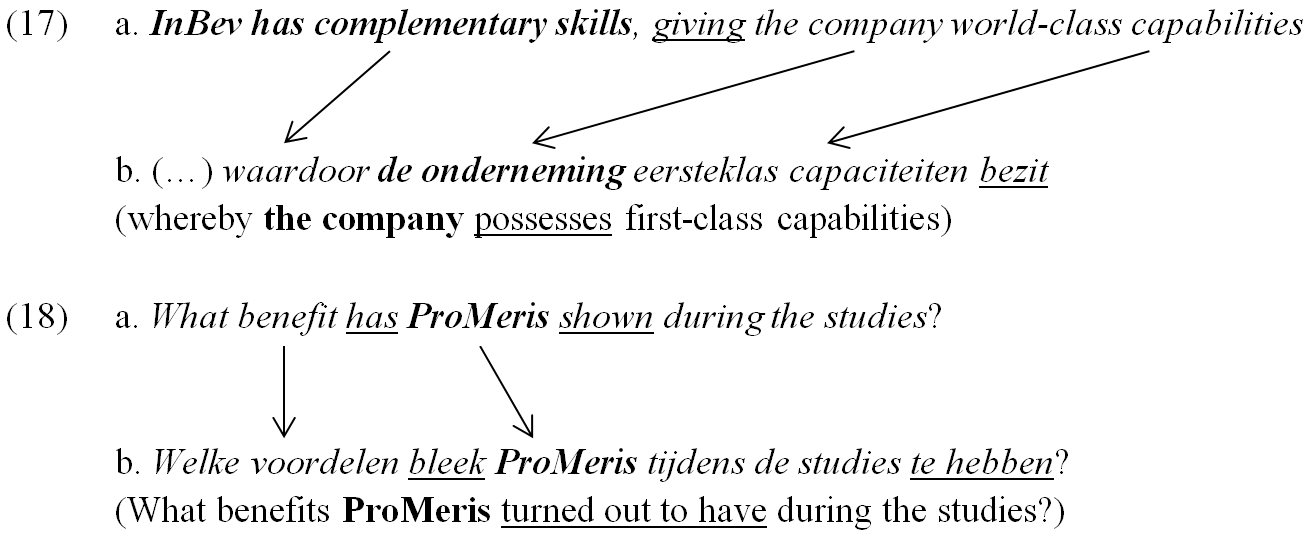
\includegraphics[width=1\textwidth]{./figures/S-7.png}
%\end{figure}


Target-text sentence (\ref{ex:5:17}b) not only differs from source-text sentence (\ref{ex:5:17}a) in the way in which \textit{give} is translated. The source-text subject which takes the form of a clause (\textit{InBev has complementary skills}) is found as the pronominal adverb \textit{waardoor} (\textit{whereby}) in Dutch, while the source-text recipient \textit{the company} becomes subject in the target text. In \REF{ex:5:18}, the source-text subject (\textit{ProMeris}) also functions as subject in Dutch, albeit as a possessor instead of a non-human agent. Further, the Dutch verb \textit{hebben} (\textit{have}) is preceded by the verb \textit{blijken} (\textit{turn out}) which adds a degree of modality to target-text sentence (\ref{ex:5:18}b). 

Finally, in almost one in ten Dutch translations of source-text sentences with \textit{give}, recipient subjects are attested. These subjects do not occur in translations of source-text sentences with \textit{show}. This might not be surprising, since verbs like \textit{krijgen} (\textit{get}) in (\ref{ex:5:19}b) actually depict the act of giving from a different angle, i.e. from the opposite perspective in which a recipient receives a theme from an agent.   

\ea \label{ex:5:19}
\ea
\textbf{People [are]} \src{smoking}{\textbf{smoking}} \textbf{behind me and that} \ul{gives} \src{me}{me} an\\\,  \src{asthma}{asthma attack}\\[1em]
\ex
Mensen achter mij zitten te \target{smoking}{roken}, waardoor \target{me}{\textbf{ik}} een\\	\, \target{asthma}{astma-aanval} \ul{krijg}\\
people behind me are smoking, whereby \textbf{I} \ul{get} an asthma attack
\z
\z

\connect{smoking}
\connect{asthma}
\connect{me}
%\begin{figure}
%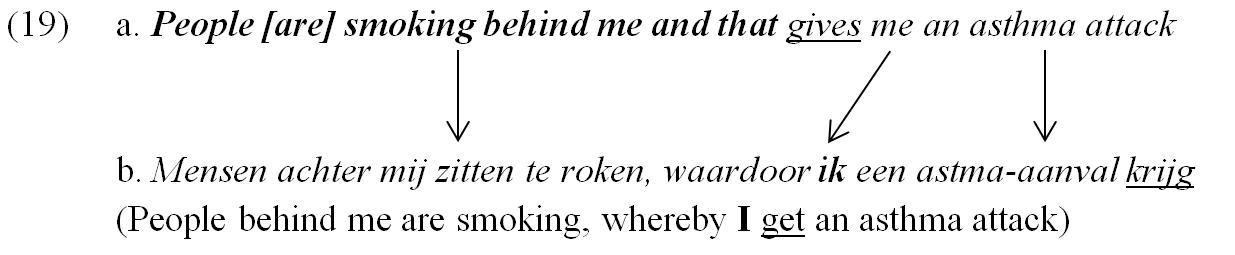
\includegraphics[width=1\textwidth]{./figures/S-8.png}
%\end{figure}

The perspective-change which takes place in \REF{ex:5:19} gives birth to the Dutch recipient subject \textit{ik} (\textit{me}) which can be brought back to the source-text recipient. The source-text subject, a non-human agent representing a clause, is portrayed in Dutch by the pronominal adverb \textit{waardoor} (\textit{whereby}) which refers to the source-text situation \textit{people [are] smoking behind me}.
  

\subsubsection{Omission of the verb} \label{sec:5:6:2:3}

A third solution to avoid Dutch non-human agents is chosen by translators in almost five percent of all Dutch translations and leads to a target-text sentence which does not contain a verb, as is illustrated in (\ref{ex:5:20}b) and (\ref{ex:5:21}b). Various ways exist through which this solution can be established. In (\ref{ex:5:20}b), the source-text verb \textit{give} is replaced in the target text with the preposition \textit{in}. This type of translation is what D’haeyere (2010) refers to as transformation into a prepositional phrase. \textit{Show}, on the other hand, is left untranslated in (\ref{ex:5:21}b). Instead, colons are introduced. In both (\ref{ex:5:20}b) and (\ref{ex:5:21}b) the lack of target-text verb engenders that no target-text subject is attested either.     


\ea \label{ex:5:20} 
\ea
(\dots) the \src{pickers}{women pickers} \textbf{whose generalised} \src{clothing}{\textbf{clothing}} \ul{gave} them a \\\,\src{timeless}{timeless} quality\\[1em]
\ex
(\dots) \target{pickers}{olijvenpluksters} in eenvoudige, \target{timeless}{tijdloze} \target{clothing}{kleding}\\
women olive pickers in simple, timeless clothing
\z
\z

\connect{pickers}
\connect{timeless}
\connect{clothing}

\ea \label{ex:5:21}
\ea
\textbf{2002} \src{results2}{\textbf{results}} \ul{shows} 11.5\% \src{oop}{organic operating profit growth}\\[1em]
\ex \target{results2}{Resultaten} 2002: interne groei \target{oop}{bedrijfsresultaat} van 11.5\%\\
results 2002: organic operating profit growth of 11.5\%
\z
\z

\connect{results2}
\connect{oop}

%\begin{figure}
%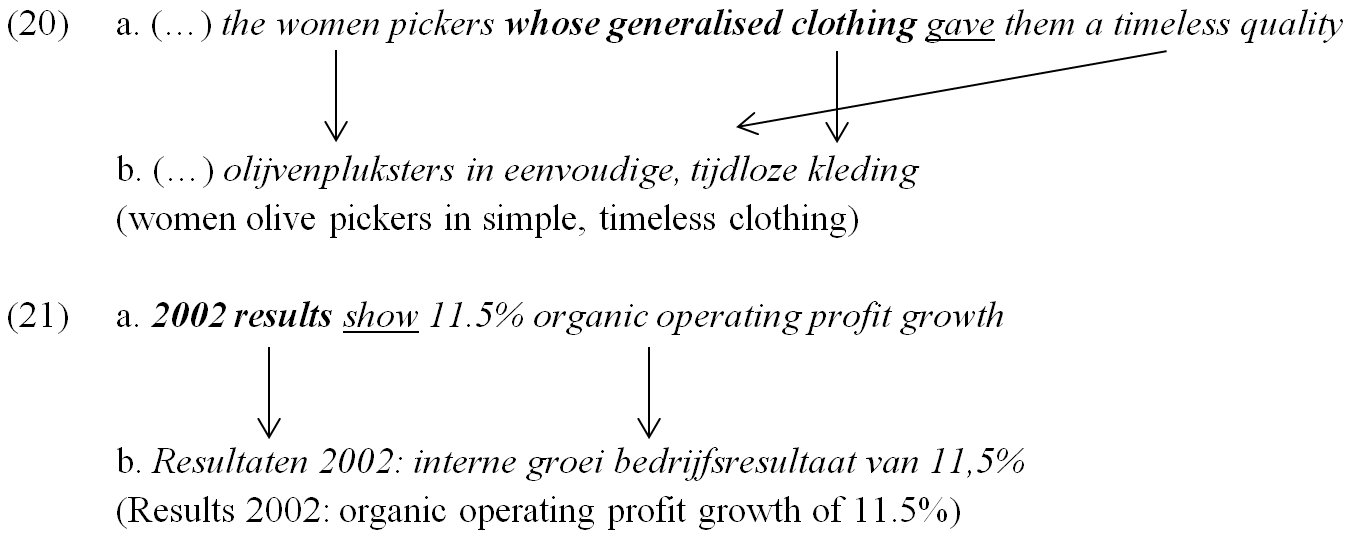
\includegraphics[width=1\textwidth]{./figures/S-9.png}
%\end{figure}


\section{Discussion}

The Dutch translations produced by translators who translated 388 English sentences with non-human agents as subjects of \textit{give} and \textit{show} seem to indicate that most lexical information stored in the source-text sentences is also displayed in the target-text sentences. Almost sixty percent of the target-text sentences contain non-human agents in subject position. In these instances, the lexical source-text information is mostly represented in word-for-word translations. In the other forty percent, however, the syntactic and semantic patterns of the source-text sentences are not followed. Nevertheless, most of these instances likewise reveal a tendency to represent the lexical information denoted by the source-text sentences throughout the Dutch translations.

In the forty percent Dutch translations in which non-human agents are avoided, especially semantic changes are attested, rather than explicitations or implicitations \citep[see][]{Vandepitte2007}. These changes in the target-text sentences often lead to differences in valency vis-à-vis the respective source texts. As the findings in \tabref{tab:5.5} show, English non-human agent subjects of \textit{give} are attested especially in trivalent (agent, theme, recipient) and only in less than third of the instances in divalent (agent and theme) source-text sentences. 	

The opposite tendency is found for the source-text sentences with non-human agent subjects of \textit{show}, which are almost exclusively divalent. This difference in the valency patterns of both source-text verbs may to some extent be brought back to their semantic nature: \textit{give} is typically referred to as a dative verb, i.e. a verb which typically takes a recipient indirect object, while \textit{show} is a lexical causative of the typically divalent verb \textit{see}, thus giving it the sense of \textit{make see}, the valency pattern of which not necessarily calls for a recipient direct object.

\begin{table}
     \centering
     \resizebox{\textwidth}{!}{
     \begin{tabular}{lllllllllll}
     \lsptoprule
     &  EN trivalent\newline \textit{give}   & \textit{\%}  & EN divalent\newline \textit{give} & \textit{\%} & EN trivalent\newline \textit{show} & \textit{\%} & EN divalent\newline \textit{show} & \textit{\%} & Total & \textit{\%} \\ \midrule
       \textbf{NL trivalent}  & 53    & 47.8      & 0	    & 0      & 2   & 40   &0    & 0    & 55  & 14.2 \\
       \textbf{NL divalent}   & 44    & 39.6      & 32      & 74.4   & 3   & 60   & 145 & 63.3 & 224 & 57.7 \\
       \textbf{NL monovalent} & 10    & 9         & 10      & 23.3   & 0   & 0    & 72  & 31.4 & 92  & 23.7 \\  
      \textbf{NL avalent}     & 4     & 3.6       & 1       & 2.3    & 0   & 0    & 12  & 5.2  & 17  & 4.4  \\ \midrule
       \textbf{Total}         & 111   & 28.6      & 43      & 11.1   & 5   & 1.3  & 229 & 59   & 388 & 100  \\ 
\lspbottomrule       
     \end{tabular}
     }
 
     \caption{Valency reduction in Dutch translations}
     \label{tab:5.5}
     % Verweis im Text mittels \REF{tbl:beispieltabelle}
 
   \end{table}

As \tabref{tab:5.5} also reveals, trivalent source-text instances of \textit{give} are translated especially with Dutch trivalent (47.8\%) and divalent (39.6\%) target-text sentences and occasionally with Dutch monovalent (9\%) and even avalent (3.6) constructions. English divalent source-text sentences of \textit{give} are translated in approximately three quarters of the instances with Dutch divalent target-text sentences and in almost a quarter of the instances with Dutch monovalent target-text sentences. The divalent source-text sentences of \textit{show} display a similar translation pattern, as they are translated in almost two thirds of the instances with Dutch divalent target-text sentences, in about a third of the instances with Dutch monovalent target-text sentences, and in some instances even with Dutch avalent constructions.

To sum up, Dutch translations of trivalent (29.9\%) and divalent (70.1\%) source-text sentences of \textit{give} and \textit{show} are mainly divalent (57.7\%) and even monovalent (23.7\%), thus indicating a valency reduction in the target-text sentences. This valency reduction, however, does not imply a loss of (lexical) information in the Dutch translations. As revealed throughout \sectref{sec:5:6:2} and its subsections, the instances in which non-human agents are avoided in Dutch show various different distributions of the source-text elements. Shifts in grammatical functions and semantic roles occur very often, giving birth to different valency patterns with regard to the source texts. These shifts, however, are usually not explicitations, nor implicitations, but semantic changes, confirming \citep{Vandepitte2007} findings.

These changes may also take the edge of \citeauthor{Delsoir2011}'s \citeyear{Delsoir2011} claim that English has been leaking into the Dutch language on a grammatical level. Perhaps, the instances in which Dutch non-human agents are maintained are the result of priming \citep[e.g.][]{Vandepitte2011,Delsoir2011} or interference from the source texts rather than an effect of the Dutch language’s drifting towards Anglo-American language norms \citep[ e.g.][]{House2008}. Or perhaps, the present findings reflect the every-day reality of translators who are faced with the problem of having to choose between a primed Dutch translation with a non-human agent in subject position and a Dutch translation without a non-human agent but with a different semantic and syntactic pattern. 

\section{Conclusion}

In this study, I have investigated how 388 English source-text sentences with non-human agents as subjects of \textit{give} and \textit{show} have been translated into Dutch. Although restrictions exist on non-human agents in subject position in Dutch, almost six in ten Dutch translations include a non-human agent. These target-text sentences follow the syntactic and semantic structure of their respective source-text sentences, which are mainly trivalent in case of sentences with \textit{give} and divalent in case of sentences with \textit{show}. On the other hand, three solutions have been proposed by translators to avoid Dutch non-human agents.

First, human agents have been introduced in less than one in ten target-text sentences. In almost a third of all Dutch translations, however, the agent is not humanized, but rather replaced with another participant which plays another semantic role such as theme, possessor or recipient. These target-text sentences are characterized by a variety of syntactic and semantic patterns which differ from the source-text patterns. These changes lead to valency reduction, but not, however, to (lexical) information loss. Finally, in some instances, the verb is omitted in the Dutch translations, so that no target-text participants can be discerned. 

Whether the present findings are the result of priming/interference or the impact English has on the Dutch language \citep[see e.g.][]{House2008,Delsoir2011} is unclear. Further research might articulate an answer to this question. It is clear, however, that translators have decided between either primed translations with non-human agents and translations without non-human agents, but with specific Dutch syntactic and semantic patterns which differ from those in the English source texts. Further research into original Dutch might also reveal whether the Dutch translations without non-human agents as well as their specific syntactic and semantic patterns are the more typical instances of the Dutch language.            

\printbibliography[heading=subbibliography,notkeyword=this]
\end{document}
